% 曲率圆
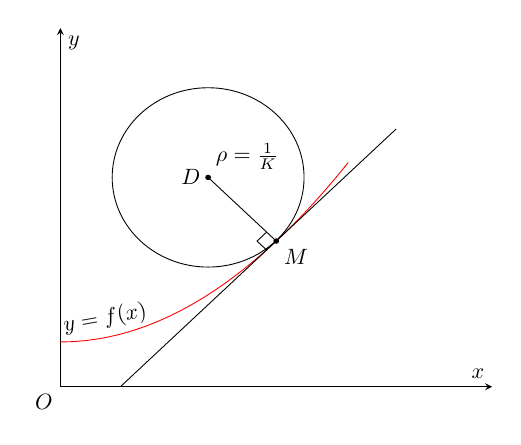
\begin{tikzpicture}[scale=0.8]
  \begin{axis}[clip=false,xmin=0, xmax=9,ymin=0,ymax=8, grid=none,
    xtick=\empty, ytick=\empty, axis lines=middle,
    smooth, xlabel={$x$}, ylabel={$y$}]

    % 曲线 y=f(x)
    % y' = 0.222 * x
    % y'' = 0.222
    \addplot[draw=red,domain=0:6] {x^2/9 + 1};

    % 弧段
    \node [above,rotate=10] at (1,1.11) {$y=f(x)$};
    \draw [fill] (4.5,3.25) circle [radius=0.05];
    \node [below right] at (4.5,3.25) {$M$};

    % 切线
    % y = x - 1.25
    \draw (1.25,0) -- (4.5,3.25) -- (7,5.75);

    % 曲率:K = 0.222 / (1+y'^2)^3/2 --> x = 4.5 --> K = 0.079
    % 半径:p = 1 / K = 12.73
    % 法线:y = -x + 7.75

    \draw [fill] (3.08,4.67) circle [radius=0.05];
    \draw (3.08,4.67) -- (4.5,3.25);
    \draw (3.08,4.67) circle [radius=2];
    \node [left] at (3.08,4.67) {$D$};
    \node [above right] at (3.08,4.67) {$\rho=\frac{1}{K}$};

    % y = -x + 7.35
    % y = x - 0.85
    \draw (4.3,3.05) -- (4.1,3.25) -- (4.3,3.45);

    % 原点
    \node [below left] at (0,0) {$O$};
  \end{axis}
\end{tikzpicture}
